\section{Обзор литературы и постановка задачи исследования}
\subsection{Реконструкция поверхности основанная на триангуляции Делоне}
В современной компьютерной графике векторно-полигональная модель является наиболее распространенной. Она применяется в системах автоматизированного проектирования, средах разработки компьютерных игр, геоинформационная системах, САПР и т. д.

Методы реконструкции поверхности основанные на триангуляции Делоне являются наиболее широко известными среди полигональных методов. Главной отличительной чертой является задание полигональной сетки треугольниками образующих граф, который обладает следующими условиями: ребра графа не пересекаются и граф обладает максимальным количеством ребер с учетом этого условия, описанная окружность для любой грани графа не содержит вершин за исключением вершин принадлежащий грани ~\cite{Скворцов}. 

\begin{figure}[h]
    \centering
    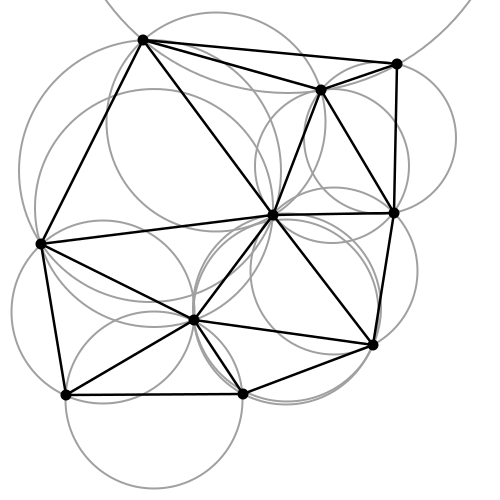
\includegraphics[scale=0.7]{images/delaunay.png}
    \caption{Выполнение инварианта триангуляции Делоне}
    \label{fig:delauney}
\end{figure}

Стоит отметить, что сами алгоритмы триангуляции не изменяют положение точек из входного облака точек. Это является слабой стороной алгоритма с точки зрения реконструкции поверхности по зашумленным входным данным. Также стоит отметить информационную зависимость алгоритмов на каждой последующей итерации от вычислений полученных на предыдущей операции, связанной с сохранением инварианта выполнения условия того, что граф является триангуляцией Делоне. Разбиение входного облака точек на сегменты ведет к последующим сложностям в соединение сегментов графа с выполнением всего того же инварианта ~\cite{Tamal}.
\subsection{Оператор локально-оптимальной проекции(LOP)}
Данный метод основан на алгоритме Вайсфельда для решения задачи Ферма-Вебера о расположении точек, также известный как многомерная медиана L1. Это статистический инструмент, который традиционно применяется во всем мире для многомерных непараметрических точечных выборок, чтобы получить хорошего представителя для большого количества выборок при наличии шума и выбросов. Эта задача была впервые сформулирована Вебером в работе ~\cite{WEBER}  под названием проблема определения оптимального местоположения. Задача состояла в том, чтобы найти оптимальное место для промплощадки, минимизирующее стоимость доступа. В статистике проблема известна как медиана L1 ~\cite{BROWN, SMALL}.

Задача Ферма-Вебера (глобальная) о расположении точек рассматривается как пространственная медиана, поскольку, будучи ограничена одномерным случаем, она совпадает с одномерной медианой и наследует некоторые ее свойства в многомерной постановке.

Реконструкция с помощью оператора проекции имеет важное достоинство: она определяет непротиворечивую геометрию на основе точек данных и предоставляет конструктивные средства для повышения ее дискретизации. 
Оператор локально-оптимальной проекции без параметризации использует более примитивный механизм проецирования, но поскольку он не основан на локальной 2D-параметризации, он более надежен и хорошо работает в сложных сценариях. Кроме того, если точки данных взяты локально с гладкой поверхности, оператор обеспечивает аппроксимацию второго порядка, что приводит к правдоподобной аппроксимации выбранной поверхности.

Оператор LOP имеет две непосредственные функции: во-первых, его можно использовать в качестве этапа предварительной обработки для любого другого метода реконструкции более высокого порядка (например, RBF). LOP можно применять к необработанным отсканированным данным для создания чистого набора данных, в качестве средства эффективного уменьшения шума и выбросов, а также для упрощения определения ориентации и топологии локальной поверхности. Во-вторых, его можно использовать для уточнения данного набора данных.

Для множества точек данных $P = \{p_j\}_{j\in J} \subset \mathbf R^{3}$, LOP проецирует произвольное множество точек $X^{(0)} = \{x_i^{(0)} \} _{i \in I} \subset \mathbf R^{3}$ на множество $P$, где $I$, $J$ обозначают наборы индексов. Множество спроецированных точек $Q = \{q_i\}_{i\in I}$ определяется так, чтобы оно минимизировало сумму взвешенных расстояний до точек P относительно радиальных весов с центром в том же множестве точек Q. Кроме того, точки Q не должны быть слишком близко друг к другу. Эта структура индуцирует определение искомых точек Q как решение уравнения с фиксированной точкой 
$$Q = G(Q),$$
где
$$G(C) = argmin_{X = \{x_i\}_{i \in I}} \{E_1(X,P,C) + E_2(X,C)\},$$
$$E_1(X,P,C) = \sum_{i \in I} \sum_{j \in J}\parallel x_i - p_j \parallel \theta(\parallel c_i - p_j \parallel), $$ 
$$E_2(X, C) = \sum _{i^{'} \in I} \lambda_{i^{'}}\sum_{i \in I \setminus\{i^{'}\}} \eta(\parallel x_{i^{'}}- c_i  \parallel)\theta(\parallel c_{i^{'}} - c_i \parallel)$$

Здесь $\theta(r)$ — быстро убывающая гладкая весовая функция с компактным опорным радиусом $h$, определяющая размер радиуса влияния, $\eta(r)$ — другая убывающая функция, штрафующая $x_{i^{'}}$ за то, что они подходят слишком близко к другим точкам, и $\{\lambda_i\}_{i \in I}$ являются уравновешивающими членами, которые обозначены через $\mathbf \land$. В двух словах, термин $E_1$ заставляет спроецированные точки $Q$ аппроксимировать геометрию $P$, а член $E_2$ стремится  сохранить справедливое распределение точек $Q$. Правильные значения $\mathbf\land$ могут гарантировать степень аппроксимации второго порядка оператора LOP при условии, что данные отбираются с поверхности $C^{2}$.

\subsection{Радиальные базисные функции(RBFs)}
Радиальные базисные функции - это хорошо известный метод интерполяции разбросанных данных. Учитывая набор точек с заданными значениями функций, RBFs воспроизводят функции, содержащие высокую степень гладкости, посредством линейной комбинации радиально-симметричных базисных функций. Для реконструкции поверхности метод ~\cite{CARR} строит поверхность, находя скалярное поле со знаком, определенное через RBFs, набор нулевых уровней которого представляет поверхность. В частности, они используют глобально поддерживаемые базисные функции $\phi : R^{+} \rightarrow R$. Затем неявная функция $\Phi$ может быть выражена как:
$$\Phi(\mathbf{x}) = g(\mathbf{x}) + \sum_j\lambda_j\phi(\parallel \mathbf{x} - \mathbf{q_j} \parallel), $$
где $g(x)$ обозначает (глобально поддерживаемый) полином низкой степени, а базисные функции сосредоточены в узлах $\mathbf{q_j} \in R^{3} $. Неизвестные коэффициенты ${\lambda}_j$ находятся путем задания интерполяционных ограничений значения функции $\theta$ при $\mathbf{p_i} \in P;$ см. рис. \ref{fig:4}. Ограничения вне поверхности необходимы, чтобы избежать тривиального решения $f (\mathbf{x}) = 0$ для $\mathbf{x} \in R^{3}$. Положительные (соответственно отрицательные) ограничения устанавливаются для точек, смещенных в точке $\mathbf{p_i}$ по $\mathbf{n_i}$ в положительном (соответственно отрицательном) направлении. Интерполяция выполняется путем объединения точек ограничения на поверхности и вне поверхности как множество центров узлов $\mathbf{q_{j}} $. Коэффициенты $\mathbf{{\lambda}_i}$ находятся с помощью плотной линейной системы с n неизвестными, эффективно вычисляемой с помощью быстрых мультипольных методов ~\cite{CARR}. Преимущество использования глобально поддерживаемых базисных функций для реконструкции поверхности заключается в том, что результирующая неявная функция является глобально гладкой. Следовательно, RBFs могут быть эффективными для создания водонепроницаемой поверхности при наличии неравномерной выборки и недостающих данных. Однако, когда входные данные содержат умеренный шум, определение правильного размещения точек вне поверхности может стать сложной задачей (см. рис. \ref{fig:4} справа). 

\begin{figure}[h]
    \centering
    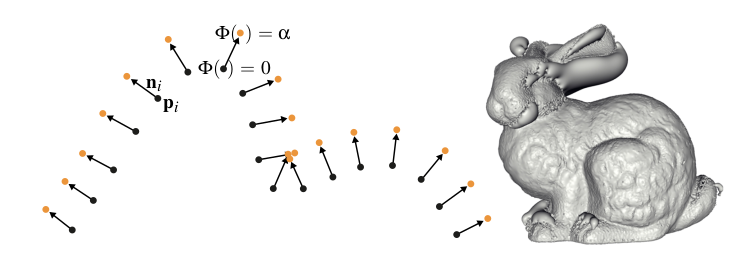
\includegraphics[scale=0.5]{images/4.png}
    \caption{(слева) Для RBFs оптимизируемое скалярное поле должно оцениваться как нуль в точках выборки $\Phi(\mathbf{p_i}) = 0$, в то время как при ограничениях вне поверхности $\Phi(\mathbf{p_i} + \alpha\mathbf{n_i}) = \alpha;$ этот выбор уместен, поскольку функции расстояния со знаком почти везде имеют норму единичного градиента. Кластер выборок вне поверхности показывает, насколько тщательно нужно задавать ограничения в областях с большой кривизной. (справа) Поверхность, реконструированная с помощью RBFs, обычно имеет серьезные геометрические и топологические артефакты, когда предоставляются противоречивые внешние ограничения.}
    \label{fig:4}
\end{figure}

\subsection{Метод движущихся наименьших квадратов}
Процедура определения поверхности методом наименьших квадратов была представлена Левином ~\cite{LEVIN}.
Пусть точки $p_i \in R^{3}, i \in \{1, . . . , N\}$, взяты с
поверхности S (возможно, с шумом измерения). Цель состоит в том, чтобы спроецировать точку $r \in R^{3}$ вблизи S на двумерную поверхность SP, аппроксимирующую $p_i$. Процедура MLS мотивирована дифференциальной геометрией, а именно тем, что поверхность может быть локально аппроксимирована функцией. Алгоритм называется движущимся, поскольку итеративно двигается по набору точек. Точка на которой находится итерация, называется точкой запроса. Для точки запроса r (см. рис. \ref{fig:0}) вычисляется локальная плоскость H с использованием метода наименьших квадратов по точкам попавшим в окрестность радиуса R (параметр алгоритма) 

Эталонная плоскость: 
 Локальная плоскость $ H = \{x \mid \langle n, x \rangle - D = 0, x  \in R^{3}\}, n \in R^{3},  \parallel n \parallel = 1 $ вычисляется так, чтобы минимизировать локальную взвешенную сумму квадратов расстояний точек $p_i$ до плоскости (см. рис. \ref{fig:0}). Веса, соответствующие $p_i$, определяются как функция расстояния от $p_i$ до проекции r на плоскость H, а не от расстояния до r. Предположим, что q является проекцией r на H, тогда H находится путем локальной минимизации
 \begin{equation}
     \sum_{i = 1}^{N}(\langle n, p_i \rangle - D)^{2} \theta(\parallel p_i - q \parallel)
     \label{eq:ref1}
 \end{equation}

где $\theta$ — гладкая монотонно убывающая функция, положительная на всем пространстве. Полагая $q = r + tn$ для некоторого $t \in R$, уравнение \ref{eq:ref1} можно переписать как: 
 $$\sum_{i = 1}^{N}(\langle n, p_i - r - tn \rangle)^{2} \theta(\parallel p_i - r - tn \parallel)$$
 
  Оператор $Q(r) = q = r + tn$ определяется как локальный минимум уравнения  с наименьшим t и локальной касательной плоскостью H вблизи r соответственно. Затем локальная эталонная область задается ортонормированной системой координат на H, так что q является началом этой системы. Затем вычисляется локальная полиномиальная аппроксимация g точек $p_i$ над H. Проекция точки запроса на полином является результатом работы алгоритма MLS.

\begin{figure}[h]
    \centering
    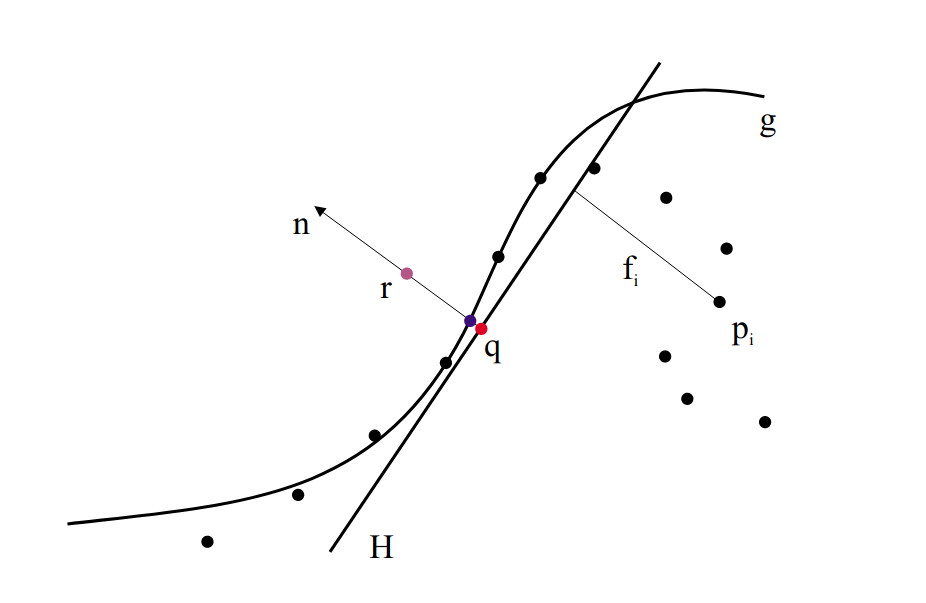
\includegraphics[scale=0.5]{images/0.png}
    \caption{Шаг алгоритма движущихся наименьших квадратов}
    \label{fig:0}
\end{figure}

\subsection{Повышение дискретизации и рендеринг}

Алгоритм MLS позволяет повысить плотность точек если плотность исходного облака точек недостаточна.  На плоскости $H$, найденной методом наименьших квадратов, задается набор точек на окружностях с заданным шагом и радиусом(см. рис. \ref{fig:upsampling}) которые в последствие проецируются на полином.

\begin{figure}[h]
  \centering
  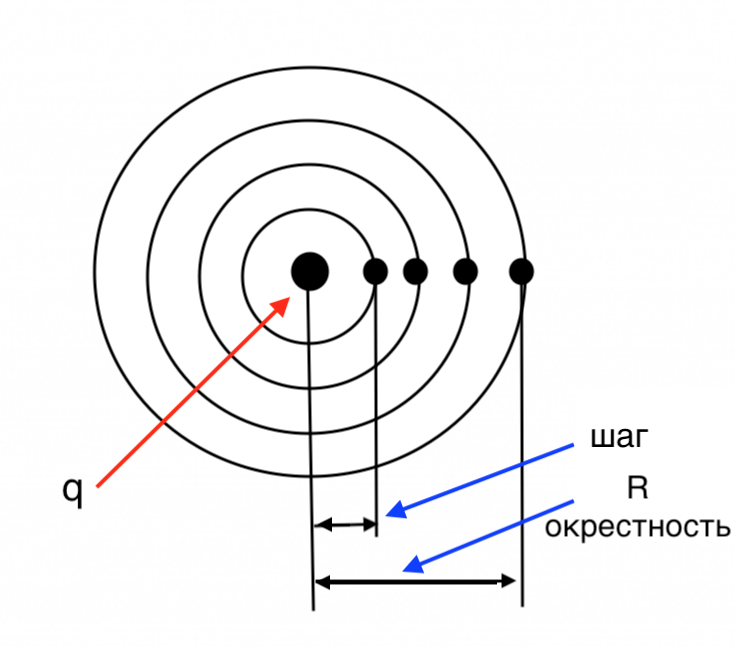
\includegraphics[width=0.42\textwidth, height=6cm]{images/rendering.png}
  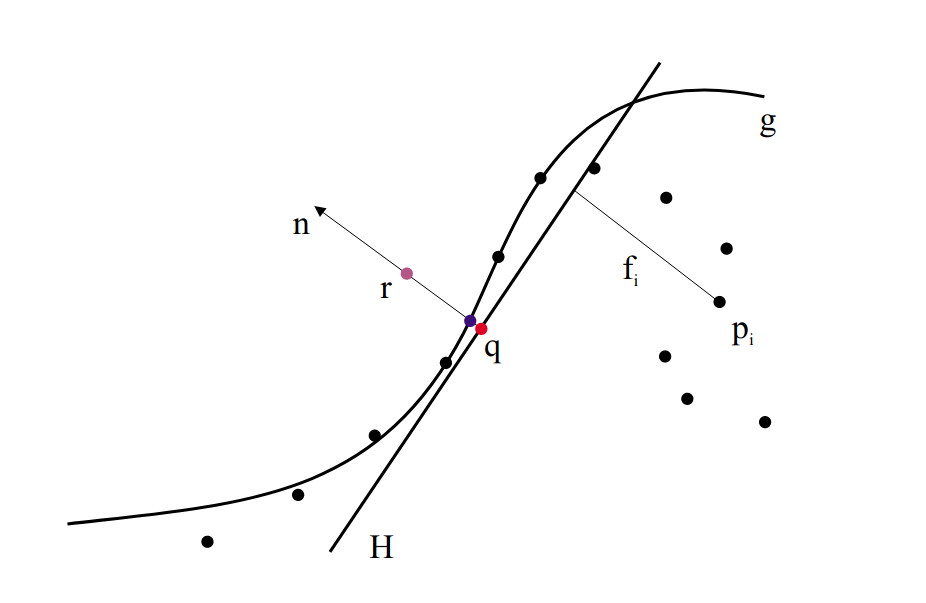
\includegraphics[width=0.56\textwidth, height=6cm]{images/0.png}
  \caption{Повышение плотности точек за счет проекции дополнительных точек выбранных на плоскости H.}
  \label{fig:upsampling}
\end{figure}

В 2000м году Шимон Русинкевич и Марк Левой предложили подход рендеринга при котором поверхность представляется набором точек и при необходимости повышается дискретизация до разрешения экрана ~\cite{Szymon}. Такой подход должен был обеспечить большую производительность ввиду отсутствия затрат на настройку и растеризацию полигонов. Но из-за значительного роста производительности графических устройств и того что рендеринг в таком программном обеспечение как Unity и Blender завязан на полигональных моделях, спустя 20 лет можно сказать что этот подход себя не оправдал.


\begin{figure}[h]
  \centering
  \subbottom[25000000 полигонов]{%
    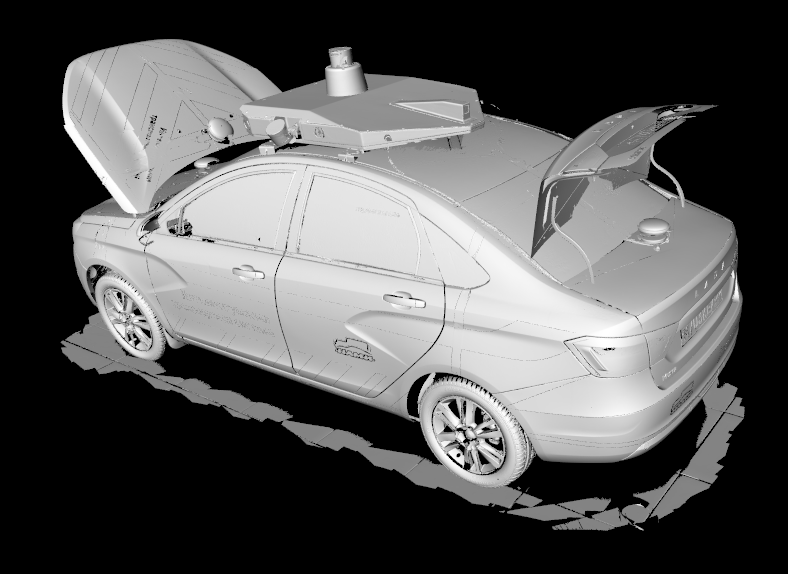
\includegraphics[width=0.49\textwidth, height=7cm]{images/polygon.png}}
  \subbottom[25000000 точек]{%
    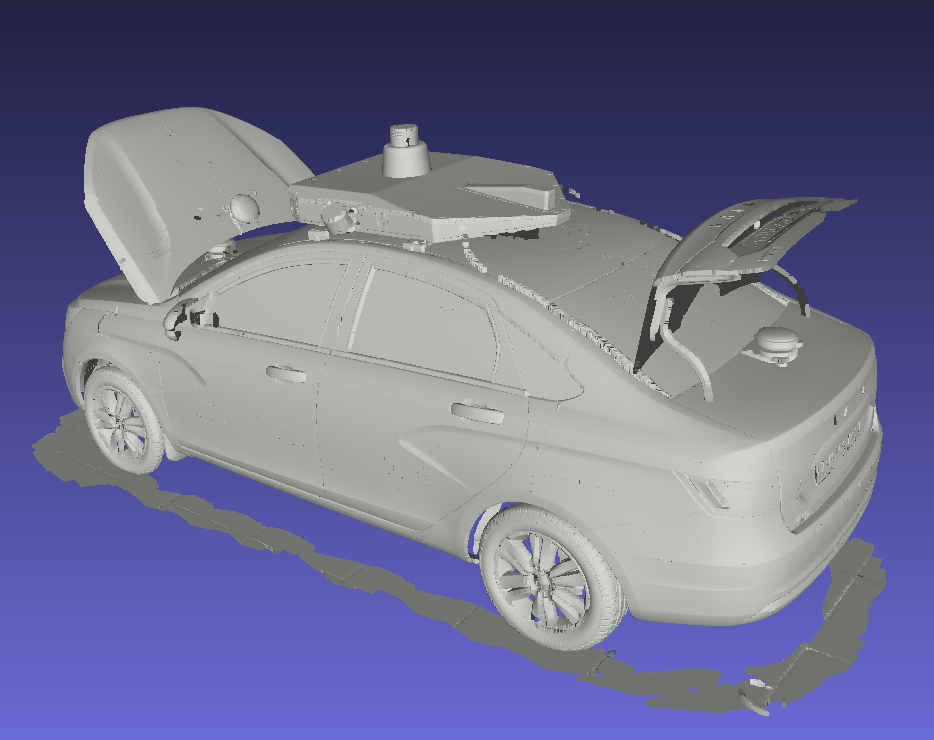
\includegraphics[width=0.49\textwidth, height=7cm]{images/point_set.png}}
  \caption{Сравнение рендеринга векторно-полигональной модели и поверхности представленной набором точек}
\end{figure}
